\chapter{Spektrale Graphentheorie}

\section{Einführung}

\begin{itemize}
  \item \emph{Spektrum} eines Graphen zur Untersuchung seiner Eigenschaften
  \item \emph{algebraische} oder \emph{spektrale Graphentheorie} genannt
\end{itemize}

Algebraische Methoden sind sehr effektiv bei Graphen, die regulär und symmetrisch sind.

\subsection{Eigenwerte, Eigenvektoren und Eigenfunktionen}

$\ma{M}\gls{eiv} = \gls{lambda}\gls{eiv}$\\
Zu einem Eigenwert $\gls{lambda}$ gibt es unendlich viele (skalierte) Eigenvektoren \gls{eiv}.
Wir definieren einen Eigenvektor \gls{eiv} dann eindeutig über $\left\|\gls{eiv}\right\|_2 = 1$.
Wenn \ma{M} symmetrisch ist und $\gls{eiv}_1$ und $\gls{eiv}_2$ zwei unterschiedliche Eigenvektoren, dann gilt $\gls{eiv}_1 \gls{ortho} \gls{eiv}_2$.
Jede symmetrische Matrix $\in \gls{R}^{n \times n}$ hat genau $n$ Eigenwerte mit $\gls{lambda}_1 \leq \cdots \leq \gls{lambda}_n$

Wir definieren $\gls{Lambda} = \gls{diag}\left(\left[\gls{lambda}_1, \ldots, \gls{lambda}_n\right]\right)$.
Wir definieren die orthogonale Matrix $\gls{Eiv} = \left[\gls{eiv}_1, \ldots, \gls{eiv}_n\right]$.
Dann gilt $\ma{M}\gls{Eiv} = \gls{Eiv}\gls{Lambda}$.
Daraus folgt sofort
\begin{equation}
  \ma{M} = \ma{M}\gls{Eiv}\gls{Eiv}^{\top} = \gls{Eiv}\gls{Lambda}\gls{Eiv}^{\top}
\end{equation}

mit $\gls{Eiv}\gls{Eiv}^{\top} = \gls{I}$.

\todo{Eigenfunktionen, brauch ich überhaupt?}

\subsection{Der Laplacian und seine Eigenwerte}

\begin{itemize}
  \item diskrete Analogie des $\nabla^2$ Operators
  \item man nimmt eine Funktion und approximiert sie mit Hilfe eines Graphen, so dass Knoten, die dichter beieinander liegen eine größere zweite Ableitung besitzen.
\end{itemize}

Der nicht-normalisierte Laplacian \gls{L} eines Graphen \gls{G} ist definiert als $\gls{L} = \gls{D} - \gls{A}$~\cite{Chung}.
Er wird auch oft kombinatorischer Laplacian genannt.
Der normalisierte Laplacian \gls{Lnorm} ist definiert als $\gls{Lnorm} = \gls{D}^{-\frac{1}{2}} \gls{L} \gls{D}^{-\frac{1}{2}}$~\cite{Chung}.
\todo{wie nennt man ihn auch?}
Es gilt die Konvention, dass ${\left(\gls{D}^{-\frac{1}{2}}\right)}_{ii} = 0$ falls $\gls{D}_{ii} = 0$ (im Falle von isolierten Knoten)
Für verbundene Graphen gilt weiterhin $\gls{Lnorm} = \gls{I} - \gls{D}^{-\frac{1}{2}} \gls{A} \gls{D}^{-\frac{1}{2}}$~\cite{Chung}.
Jeder Eintrag der Diagonalen von \gls{Lnorm} ist damit $1$.
\gls{Lnorm} ist weiterhin symmetrisch, das wäre bei einer Normierung der Form $\gls{D}^{-1}\gls{L}$ nicht der Fall.

\gls{L} und \gls{Lnorm} sind keine ähnlichen Matrizen.
Insbesondere sind ihre Eigenvektoren unterschiedlich.
Die Nutzung von \gls{L} oder \gls{Lnorm} ist damit abhängig von dem Problem, welches man betrachtet.~\cite{Hammond}.

Wir schreiben \gls{Lboth} wenn die Wahl des Laplacian \gls{L} oder \gls{Lnorm} irrelevant ist.

\subsection{Visuelle Interpretation des Laplacian}

$\nabla^2 f = \nabla \cdot \nabla f$

Die Divergenz eines Vektorfeldes ist ein Skalarfeld, das an jedem Punkt angibt, wie sehr die Vektoren in einer kleinen Umgebung des Punktes auseinanderstreben.

The Laplace operator measures how much a function differs at a point from the average of the values of the function over small spheres centered at that point. As it turns out, the Laplacian of a graph does something completely analogous: namely, it measures how much a function on a graph differs at a vertex from the average of the values of the function over the neighbors of the vertex.

Im $n$-dimensionalen euklischen Raum
\begin{equation}
  \nabla^2f = \sum_{i=1}^n \frac{\partial^2f}{\partial x^2_k}
\end{equation}
in einer Dimension reduziert sich der Laplace-Operator auf die zweite Ableitung $\nabla^2 f = f^{\prime\prime}$.

Der \emph{diskrete Laplace-Operator} ist eine Analogie zum diskreten Laplace-Operator, der finite Differenzen $x \pm h$ zur Approximation von $\nabla^2 f$ nutzt
\todo{Laplace-Operator}
\todo{diskreter Laplace-Operator} Approximation des Laplace-Operators für finite Elemente

Sei $f \colon \gls{V} \to \gls{R}$ eine Funktion auf den Knoten eines Graphen.
$f$ kann ebenso als Vektor $\ve{f} \in \gls{R}^n$ betrachtet werden mit der Ordnung der Knoten, die die Adjazenzmatrix vorgibt.

Dann gilt für \gls{Lboth}, dass
\begin{equation}
  {\left(\gls{Lboth}\ve{f}\right)}_i = \sum^n_{\substack{j=0\\j \neq i}} -\gls{Lboth}_{ij} \left(\ve{f}_i - \ve{f}_j\right)
\end{equation}

Für einen Graphen, der ein reguläres Gitter aufspannt mit gleichen Kantengewichten $\frac{1}{h^2} \in \gls{R}$ gilt für einen Knoten an Position $\left(x, y\right)$:
Abusing the index notation
\begin{equation}
  {\left(\gls{L}\ve{f}\right)}_{x,y} = \frac{4\ve{f}_{x,y} - \ve{f}_{x+1,y} - \ve{f}_{x-1,y} - \ve{f}_{x,y+1} - \ve{f}_{x,y-1}}{h^2}
\end{equation}
beschreibt die \emph{5-Punkte-Stern} Approximation $-\nabla^2 f$.
mit $\nabla^2 f$ definiert auf den fünf Punkten $\left\{\left(x,y\right), \left(x+h,y\right), \left(x-h,y\right), \left(x,y+h\right),\left(x,y-h\right)\right\}$.
\begin{equation}
  \gls{Lboth}f \approx - \nabla^2 f
\end{equation}

\todo{vertauschen, erst beispiel auf gitter, dann analog zu graphen gitter}

Damit kann der Graph Laplacian als eine Generalisierung des diskreten Laplacian auf einem Gitter verstanden werden.

Eigenwerte und Eigenvektoren werden benutzt, um zu verstehen was passiert, wenn wir einen Operator (hier \gls{Lboth}) mehrfach auf einen Vektor $\ve{x}$ anwenden (hier Merkmal auf den Knoten).

Wir können \ve{x} als Linearkombination der \emph{Eigenbasis} schreiben mit
\begin{equation}
  \ve{x} = \sum_i c_i \gls{eiv}_i
\end{equation}
und berechnen dann
\begin{equation}
  \gls{Lboth}^k \ve{x} = \sum_i c_i \gls{Lboth}^k \gls{eiv}_i = \sum_i = c_i \gls{lambda}_i \gls{Lboth}^{k-1} \gls{eiv}_i = \sum_i c_i \gls{lambda}_i^k \gls{eiv}_i
\end{equation}
Wenn wir einen Operator haben, der einen Graphen beschreibt, dann können Eigenschaften dieses Operators und damit des Graphen selber durch dessen Eigenwerte und Eigenvektoren beschrieben werden.

\subsection{Eigenschaften}

Jede Reihen- und Spaltensumme von $\gls{Lboth}$ ist $0$, d.h.\ $\sum_i \gls{Lboth}_{ij} = 0$ und $\sum_i \gls{Lboth}_{ji} = 0$ für alle $i \in \left\{1, \ldots, n\right\}$.

$\gls{Lboth} \in \gls{R}^{n \times n}$ hat genau $n$ Eigenwerte ${\left\{\gls{lambda}_i\right\}}_{i = 1}^n$, wobei die Eigenwerte für gewöhnlich aufsteigend sortiert werden, d.h.\ $\gls{lambda}_i \leq \gls{lambda}_{i+1}$.

\gls{Lboth} ist eine symmetrische reelle Matrix, d.h.\ insbesondere liegen ihre Eigenwerte $\gls{lambda}_i$ in $\gls{R+}$.
Damit ist \gls{Lboth} positiv semidefinit, d.h. $\ve{x}^{\top}\gls{Lboth}\ve{x} \geq 0$ für alle $\ve{x} \in \gls{R}^n$.\todo{quelle}

Anzahl der Eigenvektoren gleich Null ist die Anzahl an Komponenten, die ein Graph besitzt.
Insbesondere gilt $\gls{lambda}_1 = 0$, da ${\left[1, \ldots, 1\right]}^{\top} \in \gls{R}^n$ Eigenvektor von \gls{Lboth}\todo{quelle, warum gilt das}\\
$0 = \gls{lambda}_1 < \gls{lambda}_2 \leq \cdots \leq \gls{lambda}_n$ wenn Graph verbunden.\todo{quelle}\\
Für einen Graphen \gls{G} definieren wir $\gls{lambda}_{\gls{G}} := \gls{lambda}_2$ und $\gls{lambda}_{\max} := \gls{lambda}_n$
Für \gls{Lnorm} gilt $\gls{lambda}_{\max} \leq 2$\todo{quelle}

Für $\gls{Lboth}^{k}$ mit $k \in \gls{N}$ gilt ${\left(\gls{Lboth}^k\right)}_{ij} = 0$ genau dann, wenn $\gls{s}\left(v_i, v_j\right) > k$~\cite{Hammond}.
Damit beschreibt $\gls{Lboth}^k$ bildlich gesprochen die Menge an Knoten, die maximal $k$ Kanten entfernt liegen.

Eine Verschrumpfung eines Graphen \gls{G} kann beschrieben werden über zwei verschiedene Knoten $u$ und $v$ zu einem neuen Knoten $v^*$ mit
\begin{align}
  \gls{w}\left(x,v^*\right) &= \gls{w}\left(x, u\right) + \gls{w}\left(x, v\right)\\
  \gls{w}\left(v^*, v^*\right) &= \gls{w}\left(u, u\right) + \gls{w}\left(v, v\right) + 2\gls{w}\left(u,v\right)
\end{align}

Für einen Graphen \gls{G} gilt für einen Graphen $H$, der aus \gls{G} verkleinert wurde,
\begin{equation}
  \gls{lambda}_{\gls{G}} \leq \gls{lambda}_H
\end{equation}

\section{Graph-Fourier-Transformation}

Directly extending this construction to arbitrary weighted graphs is problematic, as it is unclear
how to define scaling and translation on an irregular graph.
We approach this problem by working in the spectral graph domain, i.e.\ the space of eigenfunctions of the graph Laplacian \gls{Lboth}.
This tool from spectral graph theory, provides an analogue of the Fourier transform for functions on weighted graphs.

Eigenwerte werden als Frequenz aufgefasst, die das Spektrum des Graphen beschreiben.
Die Eigenvektoren beschreiben beschreiben die Signale zu den gegebenen Frequenzen.

Fourier-Transformation beschreibt die gleiche Funktion $f$, aber in einer völlig anderen Domäne.
Nicht in der Vertex-Domäne, sondern in der Spectrum-Domäne, d.h.\ auf Basis der Eigenwerte.

Ein Signal in der Fourier-Transformierten wird daher beschrieben durch den \glqq{}Anteil\grqq\ oder die Amplituden der Eigenwerte des Graphen.\todo{das stimmt so nicht}

Fourier Transformation:
\todo{warum kann man die Fourier Transformation so definieren?}
\begin{equation}
  \ve{\hat f}_i = \hat f\left(\gls{lambda}_i\right) = \sum_{j=1}^{n} f\left(v_j\right) {\left(\gls{eiv}_i\right)}_j = \sum_{j=1}^{n} \ve{f}_j {\left(\gls{eiv}_i\right)}_j
\end{equation}
oder in Matrixschreibweise
\begin{equation}
  \ve{\hat f} = \gls{Eiv}^{\top}\ve{f}
\end{equation}

Inverse Fourier Transformation
\begin{equation}
  \ve{f}_i = f\left(v_i\right) = \sum_{j=1}^n \hat f\left(\gls{lambda}_j\right) {\left(\gls{eiv}_j\right)}_i = \sum_{j=1}^n \ve{\hat f}_j {\left(\gls{eiv}_j\right)}_i
\end{equation}
oder in Matrisschreibweise
\begin{equation}
  \ve{f} = \gls{Eiv}\ve{\hat f}
\end{equation}

Fourier-Transformation hat gute Eigenschaften (Faltung ist reine Multiplikation)
Mittels der Fouriertransformierten kann man die Faltung zweier Funktionen als Produkt ihrer Fouriertransformierten ausdrücken.

\section{Spectral Graph Domain}

\begin{itemize}
  \item \emph{Spectral Graph Domain}: Der Raum der Eigenfunktionen von $\mathcal{L}$
  \item Analogon (Nachbildung) einer \emph{Fourier-Transformation} von Funktionen auf gewichteten Graphen
\end{itemize}

Eine beliebige Funktion $f: V \rightarrow \mathbb{R}$ kann als ein Vektor in $\mathbb{R}^n$ gesehen werden.
Dies impliziert eine Ordnung auf den Knoten.
Wir schreiben $f \in \mathbb{R}^n$ für Funktionen auf den Knoten eines Graphen und $f(m)$ für den Wert des $m$ten Knoten.

Dann gilt für eine beliebige Funktion $f \in \mathbb{R}^n$

\begin{equation}
  \mathcal{L}f(x) = \sum_{x~y} w(x, y) \cdot (f(x) - f(y))
\end{equation}

wobei die Summe über $x~y$ die Summierung über alle Knoten $y$ beschreibt, die adjazent zu $x$ sind.

Angenommen $G$ ist als ein reguläres Gitter definiert der Breite und Höhe $M$
Dann hat ein Knoten $v_{x,y}$ genau 4 Nachbarn mit Kantengewicht $\frac{1}{{(\delta w)}^2}$, bei dem $\delta w$ die euklidsche Distanz zwischen zwei Gitterpunkten beschreibt.

Für eine Funktion $f: M \times M \rightarrow \mathbb{R}$ gilt dann:

\begin{equation}
  \mathcal{L}f(x, y) = \frac{4f(x,y) - f(x+1, y) - f(x-1, y) - f(x, y+1) - f(x, y-1)}{{(\delta w)}^2}
\end{equation}

Damit kann ein Signal $f$ mit der Multiplikation mit $\mathcal{L}$ als eine Weiterpropagation von $f$ unter der Berücksichtigung der lokalen Nachbarn verstanden werden (\emph{5-point Stencil}, d.h.\ $\mathcal{L}f \approx - \nabla^2 f$).

\section{Diskrete Fourier Transformation}

$\mathcal{L}$ besitzt genau $n$ orthogonal zueinander stehende Eigenvektoren $\lbrace u_l \rbrace_{l=1}^n \in \mathbb{R}^n$.
Eigenvektoren $u_i$ sind auf $1$ normiert, d.h.\ $||u_i||_2 = 1$.
Diese werden auch \emph{Graph Fourier Modes} genannt.
Diesen sind Eigenwete $\lbrace \gls{lambda}_l \rbrace_{l=1}^n \in \mathbb{R}$ zugeordnet, die die \glqq{}Frequenzen\grqq\ bzw.\ das Spektrum des Graphen beschreiben oder visuell betrachtet die Ausdehnung des Raumes, den die Eigenvektoren aufspannen.
Bemerke dass $\gls{lambda}_0 = 0$, da für den Eigenvektor $\vec{u_0} = {(1, 1, \ldots, 1)}^T$ gilt, dass $\mathcal{L}\vec{u_0} = 0$.
$\mathcal{L}$ ist diagonalisierbar über $\mathcal{L} = U \Lambda U^T$, wobei $U = [u_1, \ldots, u_n] \in \mathbb{R}^{n \times n}$ die \emph{Fourier Basis} und $\Lambda = \text{diag}([\gls{lambda}_0, \ldots, \gls{lambda}_n]) \in \mathbb{R}^{n \times n}$.
Die \emph{Fourier Transformation} eines Signals $x \in \mathbb{R}^n$ ist dann definiert als $\hat{x} = U^{T}x$ und die Inverse als $x = U\hat{x}$.

\section{Faltung}

Wir suchen einen Operator $x *_G g$, der eine Faltung zweier Eingangssignale $x, g$ zu einem Ausgangssignal umleitet.
$x$ beschreibt dabei die Knotenattribute und $g$ die Gewichte.

\subsection{Faltung in CNNs}

In der Funktionalanalysis beschreibt die \emph{Faltung} einen mathematischen Operator, der für zwei Funktion $f$ und $g$ eine dirtte Funktion $f * g$ liefert.
Die Faltung kann als ein Produkt von Funktionen vertanden werden.

Anschaulich ist $(f * g)(x)$ der \emph{gewichtete Mittelwert} von $f$, wobei die Gewichtung durch $g$ gegeben ist.

Angenommen wir wollen über einer Matrix mit einem \emph{Filter} falten.
Sei unsere Eingangsmatrix $3 \times 4$ und unsere Filtergröße $2 \times 2$.

Dann gilt zum Beispiel für den Faltungsoperator $*$ in einem Convolutional Neural Network:

\begin{equation}
  \begin{pmatrix}
    1 & 2 & 3 & 1\\
    4 & 5 & 6 & 1\\
    7 & 8 & 9 & 1
  \end{pmatrix} * \begin{pmatrix}
    1 & 1\\
    1 & 1
  \end{pmatrix} = \begin{pmatrix}
    12 & 16 & 11\\
    24 & 28 & 17
  \end{pmatrix}
\end{equation}

$f: 3 \times 4 \rightarrow \mathbb{R}$ und $g: 2 \ times 2 \rightarrow \mathbb{R}$, dann ist $*$ definiert als

\begin{equation}
  (f * g)(x, y) = \sum_{x_i \in [x, x+1]\\y_i \in [y, y+1]} f(x_i, y_i)g(x-x_i, y-y_i)
\end{equation}

\subsection{Faltung auf Graphen}

Da wir keinen Translationsoperator auf der Domäne der Knoten $x$ beschreiben können, müssen wir unseren Faltungsoperator in der Fourier-Domäne beschreiben.
Dafür wandeln wir unsere Knotenmenge $x$ zuerst in $\hat x$ um.

Wir definieren $*_G$ in der Fouier-Domäne als

\begin{equation}
  x *_G g = U \cdot (U^T \cdot x \odot \hat g)
\end{equation}

wobei $\odot(A, B) = (a_{ij} \cdot b_{ij})$ die elementweise Multiplikation bzw.\ das \emph{Hadamard-Produkt}.

Das Hadamard-Produkt löst sich auf, wenn $\hat g$ als eine Diagonalmatrix repräsentiert wird. Dann gilt

\begin{equation}
  x *_G g = U \begin{pmatrix}
    \hat g(\gls{lambda}_0) & \cdots & 0\\
    0 & \cdots & \hat g(\gls{lambda}_n)
  \end{pmatrix}U^T x = U \hat g(\Lambda) U^T x
\end{equation}

Dann beschreibt $\hat g(\Lambda) = \text{diag}(\theta)$ eine Gewichtsfunktion mit $n$ Variablen, $\theta \in \mathbb{R}^n$.
Damit ist die Faltung bzw.\ die Gewichtung abhängig von der Input-Größe $n$, was extrem schlecht ist.

\subsection{Offene Fragen}

\begin{itemize}
  \item Wie erklärt sich noch einmal der normalisierte Laplacian?
  \item Warum wird $\hat g$ als Diagonalmatrix repräsentiert?
  \item Wie kommt die Convolution zustande mit dem $*$ Operator?
  \item Was passiert bei gerichteten Graphen???? Wir haben keinen symmetrischen und insbesondere keinen positiv definiten
\end{itemize}

\section{Chebyshev Polynome}

\section{Probleme}

Rotationsinvariant

\section{Pfadlänge}

wenn $d_G(m,n) > k$, dann ${(L^k)}_{m, n} = 0$
(normalisiert sowie unnormalisiert (siehe Wavelet Lemma 5.4))

\section{Eigenwerte und Eigenvektoren reell symmetrischer Matrizen}

$\ma{M}\gls{eiv} = \gls{lambda}\gls{eiv}$\\
Zu einem Eigenwert $\gls{lambda}$ gibt es unendlich viele (skalierte) Eigenvektoren \gls{eiv}.
Wir definieren einen Eigenvektor \gls{eiv} dann eindeutig über $\left\|\gls{eiv}\right\|_2 = 1$.
Sei \ma{M} weiterhin reell symmetrisch, d.h. $\ma{M} = \ma{M}^{\top} \in \gls{R}^{n \times n}$.
Dann gilt für zwei unterschiedliche Eigenvektoren $\gls{eiv}_1$ und $\gls{eiv}_2$, dass $\gls{eiv}_1 \gls{ortho} \gls{eiv}_2$.
\ma{M} hat dann genau $n$ reelle Eigenwerte mit ${\left\{\gls{lambda}_i\right\}}_{i=1}^n$.
Wir definieren $\gls{Lambda} = \gls{diag}\left(\left[\gls{lambda}_1, \ldots, \gls{lambda}_n\right]\right)$.

Wir definieren die orthogonale Matrix $\gls{Eiv} = \left[\gls{eiv}_1, \ldots, \gls{eiv}_n\right] \in \gls{R}^{n \times n}$.
Dann gilt $\ma{M}\gls{Eiv} = \gls{Eiv}\gls{Lambda}$.
und insbesondere ist \ma{M} diagonalisierbar über
\begin{equation}
  \ma{M} = \ma{M}\gls{Eiv}\gls{Eiv}^{\top} = \gls{Eiv}\gls{Lambda}\gls{Eiv}^{\top}
\end{equation}

mit $\gls{Eiv}\gls{Eiv}^{\top} = \gls{I}$.

Damit gilt insbesondere für symmetrisch reelle Matrizen $\ma{M}$, $k \in \gls{N}$
\begin{equation}
  \ma{M}^k = {\left(\gls{Eiv}\gls{Lambda}\gls{Eiv}^{\top}\right)}^k = \gls{Eiv}\gls{Lambda}^k\gls{Eiv}^{\top}
\end{equation}

Diesen Zusammenhang kann man sicht leicht erklären, wenn man die Potenz ausschreibt:
\begin{equation}
  {\left(\gls{Eiv}\gls{Lambda}\gls{Eiv}^{\top}\right)}^k = \gls{Eiv}\gls{Lambda}\gls{Eiv}^{\top}\gls{Eiv}\gls{Lambda}\gls{Eiv}^{\top}\prod^{k-2}_{i=1} \gls{Eiv}\gls{Lambda}\gls{Eiv}^{\top} = \gls{Eiv}\gls{Lambda}^2\gls{Eiv}^{\top} \prod^{k-2}_{i=1} \gls{Eiv}\gls{Lambda}\gls{Eiv}^{\top} = \gls{Eiv}\gls{Lambda}^k \gls{Eiv}^{\top}
\end{equation}

Falls \ma{M} weiterhin \emph{schwach diagonaldominant} ist, d.h
\begin{equation}
  \sum_{j=1}^n \left|\ma{M}_{ij}\right| \leq \left|\ma{M}\right|_{ii}
\end{equation}
für alle $i \in \left\{1, \ldots, n\right\}$ sind ihre Eigenwerte $\lambda_i \in \gls{R+}$ positiv reell und wir können auf diesen eine Ordnung definieren mit $0 \leq \gls{lambda}_1 \leq \cdots \gls{lambda}_n$.
Insbesondere ist \ma{M} dann \emph{positiv-semidefinit}, das bedeutet
\begin{equation}
  \ve{x}^{\top}\ma{M}\ve{x} \geq 0
\end{equation}

\section{Der Laplacian und seine Eigenwerte}

Der \emph{kombinatorische Laplacian} \gls{L} eines Graphen \gls{G} ist definiert als $\gls{L} = \gls{D} - \gls{A}$~\cite{Chung}.
$\gls{L}$ ist eine symmetrische Matrix.

Der \emph{normalisierte Laplacian} \gls{Lnorm} ist definiert als $\gls{Lnorm} = \gls{D}^{-\frac{1}{2}} \gls{L} \gls{D}^{-\frac{1}{2}}$~\cite{Chung}.
Es gilt die Konvention, dass ${\left(\gls{D}^{-\frac{1}{2}}\right)}_{ii} = 0$ falls $\gls{D}_{ii} = 0$ (d.h.\ $v_i$ ist isolierter Knoten)

Für verbundene Graphen gilt damit $\gls{Lnorm} = \gls{I} - \gls{D}^{-\frac{1}{2}} \gls{A} \gls{D}^{-\frac{1}{2}}$~\cite{Chung}.
Jeder Eintrag der Diagonalen von \gls{Lnorm} ist damit $1$.
\gls{Lnorm} ist weiterhin symmetrisch, das wäre bei einer Normierung der Form $\gls{D}^{-1}\gls{L}$ nicht der Fall.

\gls{L} und \gls{Lnorm} sind keine ähnlichen Matrizen.
Insbesondere sind ihre Eigenvektoren unterschiedlich.
Die Nutzung von \gls{L} oder \gls{Lnorm} ist damit abhängig von dem Problem, welches man betrachtet.~\cite{Hammond}.

Wir schreiben \gls{Lboth} wenn die Wahl des Laplacian \gls{L} oder \gls{Lnorm} irrelevant ist.

\subsection{Visuelle Interpretation des Laplacian}

\begin{itemize}
  \item diskrete Analogie des $\nabla^2$ Operators
  \item man nimmt eine Funktion und approximiert sie mit Hilfe eines Graphen, so dass Knoten, die dichter beieinander liegen eine größere zweite Ableitung besitzen.
\end{itemize}


$\nabla^2 f = \nabla \cdot \nabla f$

Die Divergenz eines Vektorfeldes ist ein Skalarfeld, das an jedem Punkt angibt, wie sehr die Vektoren in einer kleinen Umgebung des Punktes auseinanderstreben.

The Laplace operator measures how much a function differs at a point from the average of the values of the function over small spheres centered at that point. As it turns out, the Laplacian of a graph does something completely analogous: namely, it measures how much a function on a graph differs at a vertex from the average of the values of the function over the neighbors of the vertex.

Im $n$-dimensionalen euklischen Raum
\begin{equation}
  \nabla^2f = \sum_{i=1}^n \frac{\partial^2f}{\partial x^2_k}
\end{equation}
in einer Dimension reduziert sich der Laplace-Operator auf die zweite Ableitung $\nabla^2 f = f^{\prime\prime}$.

Der \emph{diskrete Laplace-Operator} ist eine Analogie zum diskreten Laplace-Operator, der finite Differenzen $x \pm h$ zur Approximation von $\nabla^2 f$ nutzt
\todo{Laplace-Operator}
\todo{diskreter Laplace-Operator} Approximation des Laplace-Operators für finite Elemente

Sei $f \colon \gls{V} \to \gls{R}$ eine Funktion auf den Knoten eines Graphen.
$f$ kann ebenso als Vektor $\ve{f} \in \gls{R}^n$ betrachtet werden mit der Ordnung der Knoten, die die Adjazenzmatrix vorgibt.

Dann gilt für \gls{Lboth}, dass
\begin{equation}
  {\left(\gls{Lboth}\ve{f}\right)}_i = \sum^n_{\substack{j=0\\j \neq i}} -\gls{Lboth}_{ij} \left(\ve{f}_i - \ve{f}_j\right)
\end{equation}

Für einen Graphen, der ein reguläres Gitter aufspannt mit gleichen Kantengewichten $\frac{1}{h^2} \in \gls{R}$ gilt für einen Knoten an Position $\left(x, y\right)$:
Abusing the index notation
\begin{equation}
  {\left(\gls{L}\ve{f}\right)}_{x,y} = \frac{4\ve{f}_{x,y} - \ve{f}_{x+1,y} - \ve{f}_{x-1,y} - \ve{f}_{x,y+1} - \ve{f}_{x,y-1}}{h^2}
\end{equation}
beschreibt die \emph{5-Punkte-Stern} Approximation $-\nabla^2 f$.
mit $\nabla^2 f$ definiert auf den fünf Punkten $\left\{\left(x,y\right), \left(x+h,y\right), \left(x-h,y\right), \left(x,y+h\right),\left(x,y-h\right)\right\}$.
\begin{equation}
  \gls{Lboth}f \approx - \nabla^2 f
\end{equation}

\todo{vertauschen, erst beispiel auf gitter, dann analog zu graphen gitter}

Damit kann der Graph Laplacian als eine Generalisierung des diskreten Laplacian auf einem Gitter verstanden werden.

Eigenwerte und Eigenvektoren werden benutzt, um zu verstehen was passiert, wenn wir einen Operator (hier \gls{Lboth}) mehrfach auf einen Vektor $\ve{x}$ anwenden (hier Merkmal auf den Knoten).

Wir können \ve{x} als Linearkombination der \emph{Eigenbasis} schreiben mit
\begin{equation}
  \ve{x} = \sum_i c_i \gls{eiv}_i
\end{equation}
und berechnen dann
\begin{equation}
  \gls{Lboth}^k \ve{x} = \sum_i c_i \gls{Lboth}^k \gls{eiv}_i = \sum_i = c_i \gls{lambda}_i \gls{Lboth}^{k-1} \gls{eiv}_i = \sum_i c_i \gls{lambda}_i^k \gls{eiv}_i
\end{equation}
Wenn wir einen Operator haben, der einen Graphen beschreibt, dann können Eigenschaften dieses Operators und damit des Graphen selber durch dessen Eigenwerte und Eigenvektoren beschrieben werden.

\subsection{Eigenschaften}

\gls{Lboth} ist eine reell symmetrische, schwach diagonaldominante Matrix und damit insbesondere positiv semidefinit.

$\gls{Lboth} \in \gls{R}^{n \times n}$ hat genau $n$ Eigenwerte ${\left\{\gls{lambda}_i\right\}}_{i = 1}^n \in \gls{R+}$ mit $\gls{lambda}_i \leq \gls{lambda}_{i+1}$.

Anzahl der Eigenvektoren gleich Null ist die Anzahl an Komponenten, die ein Graph besitzt.

Insbesondere sind jede Reihen- und Spaltensumme von $\gls{Lboth}$ ist $0$, d.h.\ $\sum_j \gls{Lboth}_{ij} = 0$ und $\sum_j \gls{Lboth}_{ji} = 0$ für alle $i \in \left\{1, \ldots, n\right\}$.
Insbesondere gilt $\gls{lambda}_1 = 0$, da $\gls{eiv}_1 = \frac{1}{\sqrt{n}}{\left[1, \ldots, 1\right]}^{\top} \in \gls{R}^n$ Eigenvektor von \gls{Lboth} mit $\gls{Lboth}\gls{eiv}_1 = 0$.\\

$0 = \gls{lambda}_1 < \gls{lambda}_2 \leq \cdots \leq \gls{lambda}_n$ wenn Graph verbunden.\todo{quelle}\\

\todo{was sagt $\gls{lambda}_2$ aus?}
Für einen Graphen \gls{G} definieren wir $\gls{lambda}_{\gls{G}} := \gls{lambda}_2$ und $\gls{lambda}_{\max} := \gls{lambda}_n$
Für \gls{Lnorm} gilt $\gls{lambda}_{\max} \leq 2$\todo{quelle}

Für $\gls{Lboth}^{k}$ mit $k \in \gls{N}$ gilt ${\left(\gls{Lboth}^k\right)}_{ij} = 0$ genau dann, wenn $\gls{s}\left(v_i, v_j\right) > k$~\cite{Hammond}.
Damit beschreibt $\gls{Lboth}^k$ bildlich gesprochen die Menge an Knoten, die maximal $k$ Kanten entfernt liegen.

Eine Verschrumpfung eines Graphen \gls{G} kann beschrieben werden über zwei verschiedene Knoten $u$ und $v$ zu einem neuen Knoten $v^*$ mit
\begin{align}
  \gls{w}\left(x,v^*\right) &= \gls{w}\left(x, u\right) + \gls{w}\left(x, v\right)\\
  \gls{w}\left(v^*, v^*\right) &= \gls{w}\left(u, u\right) + \gls{w}\left(v, v\right) + 2\gls{w}\left(u,v\right)
\end{align}

Für einen Graphen \gls{G} gilt für einen Graphen $H$, der aus \gls{G} verkleinert wurde~\cite{Chung},
\begin{equation}
  \gls{lambda}_{\gls{G}} \leq \gls{lambda}_H
\end{equation}

\section{Faltung mittels Graph-Fourier-Transformation}

\subsection{Kontinuierliche Fourier-Transformation}

kontinuierliche oder klassische Fourier-Transformation:
Konvertierung eines Signals in dessen Frequenzspektrum
Signal $f \colon \gls{R} \to \gls{R}$

Die komplexe Exponentialfunktion $\exp\left(\mathrm{i}\omega t\right)$ der Fourier-Transformation beschreibt die \emph{Eigenfunktionen} des eindimensionalen Laplace-Operators $\nabla^2$.
\todo{das verstehe ich nicht}

Die inverse Fourier-Transformation
\begin{equation}
  f\left(t\right) = \frac{1}{2\pi} \int \hat f\left(\omega\right) \exp\left(\mathrm{i}\omega t\right)\,\mathrm{d}\omega
\end{equation}
kann damit als die Ausdehnung von $f$ in Bezug auf die Eigenfunktionen des Laplace-Operators gesehen werden.

\subsection{Graph-Fourier-Transformation}

Wir können die \emph{Graph-Fourier-Transformation} analog dazu definieren.\\
Eigenwerte beschreiben die Frequenzen des Graphen.

Signal $f \colon \gls{V} \to \gls{R}$ auf Graphen\\
Signal kann ebenso als Vektor $\ve{f} \in \gls{R}^n$ aufgefasst werden (impliziert Ordnung der Knoten, ist durch Adjazenzmatrix gegeben)\todo{schon weiter oben definiert, eher in grundlagen unterbringen?}\\
\begin{equation}
  \hat f(\gls{lambda}_i) = \left\langle \ve{f}, \gls{eiv}_i \right\rangle
\end{equation}
bzw.\ als Vektor
\begin{equation}
  \ve{\hat f} = \gls{Eiv}^{\top} \ve{f}
\end{equation}

Die inverse Transformation ist dann definiert als
\begin{equation}
  f\left(v_i\right) = \sum_{j=1}^n \hat f\left(\gls{lambda}_j\right) {\left(\gls{eiv}_j\right)}_i
\end{equation}
bzw.\ als Vektor
\begin{equation}
  \ve{f} = \gls{Eiv}\ve{\hat f}
\end{equation}

\todo{parseval relation?}

Spectral Graph Domain

\begin{itemize}
  \item \emph{Spectral Graph Domain}: Der Raum der Eigenfunktionen von $\mathcal{L}$
  \item Analogon (Nachbildung) einer \emph{Fourier-Transformation} von Funktionen auf gewichteten Graphen
\end{itemize}

Das ermöglicht uns das Anwenden verschiedener Operation wie Filterung, Translation oder Faltung.\todo{quelle}

Directly extending this construction to arbitrary weighted graphs is problematic, as it is unclear
how to define scaling and translation on an irregular graph.
We approach this problem by working in the spectral graph domain, i.e.\ the space of eigenfunctions of the graph Laplacian \gls{Lboth}.
This tool from spectral graph theory, provides an analogue of the Fourier transform for functions on weighted graphs.

Eigenwerte werden als Frequenz aufgefasst, die das Spektrum des Graphen beschreiben.
Die Eigenvektoren beschreiben beschreiben die Signale zu den gegebenen Frequenzen.\todo{mmh}

Fourier-Transformation beschreibt die gleiche Funktion $f$, aber in einer völlig anderen Domäne.
Nicht in der Vertex-Domäne, sondern in der Spectrum-Domäne, d.h.\ auf Basis der Eigenwerte.

In classical Fourier analysis, the eigenvalues carry a specific notion of frequency:
for $\omega$ close
to zero (low frequencies), the associated complex exponential
eigenfunctions are smooth, slowly oscillating functions,
whereas for $\omega$ far from zero (high frequencies), the associated
complex exponential eigenfunctions oscillate much more
rapidly. In the graph setting, the graph Laplacian eigenvalues
and eigenvectors provide a similar notion of frequency. For
connected graphs, the Laplacian eigenvector u0 associated
with the eigenvalue 0 is constant and equal to 1
at each
vertex. The graph Laplacian eigenvectors associated with low
frequencies $\gls{lambda}_2$ vary slowly across the graph; i.e., if two
vertices are connected by an edge with a large weight, the
values of the eigenvector at those locations are likely to be
similar. The eigenvectors associated with larger eigenvalues
oscillate more rapidly and are more likely to have dissimilar
values on vertices connected by an edge with high weight.

Graph Fourier Transformation und ihre Inverse gibt uns die Möglichkeit, ein Signal in zwei verschiedenen Domänen zu repräsentieren, nämlich die Knotendomäne (das unveränderte Signal auf der Knotenmenge $\ve{f}$) und der spektralen Domäne (das transformierte Signal in das Spektrum des Graphen).
Signale, die im Spektrum definiert werden, werden \emph{Kernel} genannt.\todo{ok?}

Die Fourier-Transformation wird unter anderem gerne genutzt, da sie gute Eigenschaften hat.

\todo{bilder bzw.\ grafiken}

\subsection{Faltung}

Es ist schwierig, Faltung auf Graphen zu definieren (wir haben keinen Translationsoperator $\left(x - t\right)$).
In der Fourier-Domäne ist dies aber sehr einfach.

In der Signalverarbeitung versteht man unter der Frequenzfilterung die Transformation eines Signals in die Fourier-Domäne und der verstärkenden oder dämpfenden Veränderung der Amplituden der Frequenzkomponenten.

Formal betrachtet also
\begin{equation}
  \hat f_{\mathrm{out}}\left(\omega\right) = \hat f_{\mathrm{in}}\left(\omega\right)\hat g\left(\omega\right)
\end{equation}

Es lässt sich zeigen, dass die Multiplikation in der Fourier-Domäne äquivalent ist zu einer Faltung in der Zeitdomäne \todo{quelle}
\begin{equation}
  f_{\mathrm{out}}\left(t\right) = \left(f_{\mathrm{in}} \star g\right)\left(t\right)
\end{equation}

Wir können das spektrale Graphfilterung analog definieren mit
\begin{equation}
  \hat f_{\mathrm{out}}\left(\gls{lambda}_i\right) = \hat f_{\mathrm{in}}\left(\gls{lambda}_i\right)\hat g\left(\lambda_i\right)
\end{equation}

Damit entspricht die Faltung eines Signals auf einem Graphen der elementweisen Multiplikation in der Spectral Graph Domain
\begin{equation}
  \ve{f}_{\mathrm{out}} = \ve{f}_{\mathrm{in}} \star \ve{g} = \gls{Eiv}\left(\gls{Eiv}^{\top}\ve{f}_{\mathrm{in}} \gls{hadamard} \gls{Eiv}^{\top}\ve{g}\right)
\end{equation}

Das lässt sich in Matrixschreibweise (die zweite obrige Formel) umschreiben über
\begin{equation}
  \ve{\hat f}_{\mathrm{out}} = \hat g\left(\gls{Lambda}\right) \ve{\hat f}_{\mathrm{in}} = \hat g\left(\gls{Lambda}\right)\gls{Eiv}^{\top}\ve{f}_{\mathrm{in}}
\end{equation}
bzw.
\begin{equation}
  \ve{f}_{\mathrm{out}} = \gls{Eiv}\hat g\left(\gls{Lambda}\right)\gls{Eiv}^{\top}\ve{f}_{\mathrm{in}}
\end{equation}
mit $\hat g\left(\gls{Lambda}\right) = \gls{diag}\left({\left[\hat g\left(\gls{lambda}_1\right), \ldots, \hat g\left(\gls{lambda}_n\right)\right]}^{\top}\right)$

\section{Polynomielle Approximation}

\begin{itemize}
  \item not localized in Space \todo{was bedeutet das?}
  \item \todo{was bedeutet $k$-localized?}
  \item Learning Komplexität linear zu der Dimension der Daten $n$
\end{itemize}

Wenn wir $\hat g\left(\gls{lambda}_i\right)$ als ein Polynom vom Grad $k$ approximieren, d.h.\

\begin{equation}
  \hat g^{\prime}(\gls{lambda}_i) = \sum_{j=0}^k c_j \gls{lambda}_i^j
\end{equation}
bzw.
\begin{equation}
  \hat g^{\prime}\left(\gls{Lambda}\right) = \sum_{j = 0}^k c_j \gls{Lambda}^j
\end{equation}
mit Koeffizienten $c_0, \ldots, c_k \in \gls{R}$, dann lässt sich der Filterungsprozess in der Spectral Graph Domain erstaunlich gut auch in der Knotendomäne interpretieren.

Der Term $\gls{Eiv}\hat g^{\prime}\left(\gls{Lambda}\right)\gls{Eiv}^{\top}$ kann dann weiter vereinfacht werden:
\begin{equation}
  \hat g^{\prime}\left(\gls{Lboth}\right) =: \gls{Eiv}\hat g^{\prime}\left(\gls{Lambda}\right)\gls{Eiv}^{\top} = \gls{Eiv} \sum_{j=0}^k c_j \gls{Lambda}^j \gls{Eiv}^{\top} = \sum_{j=0}^k c_j \gls{Eiv}\gls{Lambda}^j\gls{Eiv}^{\top} = \sum_{j=0}^k c_j \gls{Lboth}^j
\end{equation}

Das sieht man leicht mit der Beziehung $\gls{Lboth}^k = {\left(\gls{Eiv}\gls{Lambda}\gls{Eiv}^{\top}\right)}^k = \gls{Eiv}\gls{Lambda}^k\gls{Eiv}^{\top}$.\todo{bereits weiter oben definiert}

Dann ist die Faltung definiert als
\begin{equation}
  \ve{f}_{\mathrm{out}} = \hat g^{\prime}\left(\gls{Lboth}\right)\ve{f}_{\mathrm{in}}
\end{equation}
bzw.
\begin{equation}
  f_{\mathrm{out}}\left(v_i\right) = \sum_{j=0} f_{\mathrm{in}}\left(v_j\right) {\left(\hat g^{\prime}\left(\gls{Lboth}\right)\right)}_{ij}
\end{equation}
Wir erinnern uns, dass ${\left(\gls{L}^l\right)}_{ij} = 0$, wenn die kürzeste Pfadlänge $\gls{s}\left(v_i, v_j\right) > l$ von $v_i$ zu $v_j$, d.h.\ die minimale Anzahl an Kanten, größer ist als $l$.

Damit kann die Faltung in der Knotenmenge intuitiv beschrieben werden als eine gewichtete Aufsummierung bzw.\ lineare Kombination der Knotensignale in einer $k$-lokalisierten\todo{definieren} Nachbarschaft um einen Knoten $v_i$
\begin{equation}
  f_{\mathrm{out}}\left(v_i\right) = f_{\mathrm{in}}\left(v_i\right) {\left(\hat g^{\prime}\left(\gls{Lboth}\right)\right)}_{ii} + \sum_{v_j \in \mathcal{N}\left(v_i, k\right)} f_{\mathrm{in}}\left(v_j\right) {\left(\hat g^{\prime}\left(\gls{Lboth}\right)\right)}_{ij}
\end{equation}

\section{Tschebyschow-Polynome}

\begin{itemize}
  \item bisheriger Ansatz skaliert nicht gut für große Graphen
  \item schneller Algorithmus zur Approximation des Filters notwendig $\Rightarrow$ Polynome niedriger Ordnung
  \item Größe des Filters soll unahängig zu den Daten sein
  \item approximiere $g(\mathcal{L})$ durch Polynom, dass rekursiv durch $\mathcal{L}$ berechnet werden kann
\end{itemize}

Diese Polynome formen eine Orthogonalbasis
\todo{stable recurrence property}
Polynome formen eine Orthogonalbasis für $L^2 \left([-1, 1], \frac{d_x}{\sqrt{1-x^2}}\right)$, auch \emph{Hilbertraum} genannt

Spektrale Filter, die repräsentiert werden durch ein Polynom vom Grad $k$ sind \emph{$k$-lokalisiert}.

\todo{die Grundidee der Polynomialsierung muss hierhin + übergang zu Chebyshev}

\subsection{Tschebyschow-Polynome}

\begin{itemize}
  \item bisher Filterung eines Signals $\mathbf{x}$ zu $\mathbf{y} = \mathbf{U}g_{\mathbf{\theta}}\left(\mathbf{\Lambda}\right)\mathbf{U}^{\top}\mathbf{x}$
  \item $g_{\mathbf{\theta}}\left(\mathbf{\Lambda}\right)$ kann über ein Polynom $k$ten Grades $g^{\prime}_{\mathbf{\theta}^{\prime}}\left(\mathbf{\Lambda}\right)$ approximiert werden, $\mathbf{\theta}^{\prime} \in \mathbb{R}^k$
  \item \underline{Aber:} Filterung ist sehr teuer aufgrund der Multiplikation der dichten Matrix $\mathbf{U}$, d.h.\ $\mathcal{O}\left(n^2\right)$
  \item \underline{Lösung:} Parametrisiere $g_{\mathbf{\theta}}\left(\mathbf{L}\right)$ als eine polynomielle Funktion, die rekursiv aus $\mathbf{L}$ berechnet werden kann.
  \item Warum sollte das effizienter sein? $\mathbf{L}$ ist nicht dicht besetzt, und hat nur $\left|\mathcal{E}\right| + n \ll n^2$ Einträge mit $n \leq \left|\mathcal{E}\right|$
\end{itemize}

\emph{Tschebyschow-Polynome} (engl. \emph{Chebyshev}) bezeichnen eine Menge von Polynomen $T_n\left(x\right) \colon \gls{R} \to \gls{R}$ mit dem rekursiven Zusammenhang
\begin{equation}
  T_n\left(x\right) = 2x T_{n-1}\left(x\right) - T_{n-2}\left(x\right)
\end{equation}
mit $T_0\left(x\right) = 1$ und $T_1\left(x\right) = x$.
Ein Tschebyschow-Polynom $T_n$ ist ein Polynom $n$-ten Grads.

Für $x \in \left[-1, 1\right]$ gilt $T_k\left(x\right) \in \left[-1, 1\right]$
\todo{irgendwas mit Hilbertraum}

Rescale $\mathbf{\Lambda}$ zu $\mathbf{\tilde \Lambda} = \frac{2}{\lambda_{\max}} \mathbf{\Lambda} - \mathbf{I} \in {\left[-1, 1\right]}^{n \times n}$.
$\lambda_{\max}$ ist der Wert des größten Eigenvektors von $\mathbf{L}$.

Dann ist $T_k\left(\mathbf{\tilde \Lambda}\right) \in {\left[-1, 1\right]}^{n \times n}$

Hammon et al zeigen, dass $g_{\mathbf{\theta}}(\mathbf{\Lambda})$ beliebig genau mit Hilfe der  rekursiven Tschebyschow-Polynome mit Grad $k$ und einer festen Filtergröße $\mathbf{\theta}^{\prime} \in \mathbb{R}^k$ approximiert werden kann
\begin{equation}
  g_{\mathbf{\theta}}\left(\mathbf{\Lambda}\right) \approx g^{\prime}_{\mathbf{\theta}^{\prime}}\left(\mathbf{\Lambda}\right) = \sum_{i = 0}^{k-1} \mathbf{\theta}^{\prime}_i T_i \left(\mathbf{\tilde \Lambda}\right)
\end{equation}

\todo{Beweisidee nachgucken}

Es zeigt sich, dass
\begin{equation}
  \mathbf{U} g^{\prime}_{\mathbf{\theta}^{\prime}}\left(\mathbf{\Lambda}\right) \mathbf{U}^{\top} = g^{\prime}_{\mathbf{\theta}^{\prime}}\left(\mathbf{L}\right)
\end{equation}

wobei $g^{\prime}_{\mathbf{\theta}^{\prime}}\left(\mathbf{L}\right) = \sum_{i=0}^{k-1} \mathbf{\theta}_i T_i\left(\mathbf{\tilde L}\right)$ mit $\mathbf{\tilde L} = \frac{2}{\lambda_{\max}}\mathbf{L} - \mathbf{I}$

Beweisidee: $\mathbf{L}^k = {\left(\mathbf{U}\mathbf{\Lambda}\mathbf{U}^{\top}\right)}^k = \mathbf{U}\mathbf{\Lambda}^k\mathbf{U^{\top}}$~\cite{GCN} und $\mathbf{U}\mathbf{U}^{\top} = \mathbf{I}$ (Quelle)
\todo{nachrechnen}

Jetzt lässt sich $y = g^{\prime}_{\mathbf{\theta^{\prime}}}\left(\mathbf{L}\right) \mathbf{x} = \sum_{i=0}^{k-1} \mathbf{\theta}^{\prime}_i T_i \left(\mathbf{\tilde L}\right) \mathbf{x}$ sehr schnell berechnen:

\begin{enumerate}
  \item berechnne $\mathbf{\overline{x}}_i$ für alle $i \in \left\{ 0, 1, \ldots, k-1 \right\}$ mit Hilfe von Rekursion:
  \begin{enumerate}
    \item $\mathbf{\overline{x}}_0 = \mathbf{x}$
    \item $\mathbf{\overline{x}}_1 = \mathbf{\tilde L} \mathbf{x}$
    \item $\mathbf{\overline{x}}_i = 2\mathbf{\tilde L} \mathbf{\overline{x}}_{i-1} - \mathbf{\overline{x}}_{i-2}$
  \end{enumerate}
\item berechne $\mathbf{y} = \left[\mathbf{\overline{x}}_0, \mathbf{\overline{x}}_1, \ldots, \mathbf{\overline{x}}_{k-1} \right] \mathbf{\theta}^{\prime}$
\end{enumerate}

\subsubsection{Laufzeit}

 \begin{itemize}
   \item anstatt $\mathbf{L}^k$ zu berechnen mit Komplexität $\mathcal{O}\left(n^2\right)$ haben wir nur noch $k$ Multiplikationen mit der Matrix $\mathbf{\tilde L}$
   \item da $\mathbf{\tilde L}$ für große Graphen sehr dünnbesetzt ist, d.h.\ $\left|\mathcal{E}\right| \ll n^2$, haben wir bei Verwendung von \emph{dünnbesetzten Matrizen} nur noch eine Laufzeit von $\mathcal{O}\left(k\left|\mathcal{E}\right|\right)$~\cite{Hammond, Defferrard}
   \item für den zweiten Schritt gilt $\mathcal{O}\left(kn\right)$, mit $n \leq \left|\mathcal{E}\right|$ bedingt damit nur Schritt Eins die Laufzeit
 \end{itemize}

\section{Graph Convolutional Networks}
\label{graph_convolutional_networks}

\citeauthor{gcn} motivieren einen weiteren Ansatz zur Faltung auf Graphen, genannt \emph{\gls{GCN}}, der auf der Methodik des spekralen Faltungsoperators aus Kapitel~\ref{spektraler_faltungsoperator} aufbaut und dabei wie eine \enquote{differenzierbare und parametrisierte Generalisierung des eindimensionalen Weisfeiler-Lehman Algorithmus auf Graphen} fungiert~\cite{gcn}.

\paragraph{Faltungsoperator}
\label{gcn_faltungsoperator}

Sei $\ve{f}_{\mathrm{in}} \star \ve{\hat g} \approx \sum_{k=0}^K c_k \gls{T}_k\left(\gls{Lbothtilde}\right) \ve{f}_{\mathrm{in}}$ der in~\eqref{eq:tschebyschow_faltung_L} definierte spektrale Faltungsoperator mit $K=1$.
Dann ist $\ve{f}_{\mathrm{in}} \star \ve{\hat g}$ eine lineare Funktion \bzgl{} \gls{Lboth} und damit eine lineare Funktion auf dem Spektrum des Graphen~\cite{gcn}.
Mit $K=1$ betrachtet der spektrale Faltungsoperator nur noch die lokale Nachbarschaft eines jeden Knotens (\vgl{}~\ref{polynomielle_approximation}).
Es ist anzumerken, dass dies in der Regel keinen Nachteil darstellt.
So hat es sich bei gegenwärtigen \enquote{State-of-the-Art}-\glspl{CNN} auf Bildern ebenfalls eingebürgert, nur noch über minimale $3\times3$ Filtergrößen zu falten und stattdessen Merkmale weit entfernterer Knoten über die mehrfache Aneinanderreihung der Faltungsschichten mittels tieferer Netze zu gewinnen~(\vgl{}~\cite{gcn, vgg, He}).
Unter dieser Restriktion vereinfacht sich $\ve{f}_{\mathrm{in}} \star \ve{\hat g}$ zu
\begin{equation}
  \ve{f}_{\mathrm{in}} \star \ve{\hat g} \approx c_0\, \ve{f}_{\mathrm{in}} + c_1 \left(\frac{2}{\gls{lambdamax}}\gls{Lboth} - \gls{I}\right)\ve{f}_{\mathrm{in}}
  \label{eq:gcn_faltung_both}
\end{equation}
mit zwei freien Parametern $c_0$ und $c_1$~\cite{gcn}.
Für $\gls{Lnorm}$ auf einem zusammenhängenden Graphen \gls{G} gilt dann nach~\eqref{eq:gcn_faltung_both} weiter
\begin{equation}
  \ve{f}_{\mathrm{in}} \star \ve{\hat g} \approx c_0 \, \ve{f}_{\mathrm{in}} + c_1 \left(\gls{Lnorm} - \gls{I}\right)\ve{f}_{\mathrm{in}} = c_0 \, \ve{f}_{\mathrm{in}} - c_1 \gls{D}^{-\frac{1}{2}} \gls{A} \gls{D}^{-\frac{1}{2}} \ve{f}_{\mathrm{in}},
  \label{eq:gcn_faltung_norm}
\end{equation}
wobei $\gls{lambdamax} \coloneqq 2$ auf dessen obere Schranke gesetzt wird~\cite{gcn}.
Um die Gefahr des Overfittings und die Anzahl an Berechnungen pro Schicht weiter zu beschränken, reduziert sich~\eqref{eq:gcn_faltung_norm} mit einem einzigen Parameter $c \coloneqq c_0$ mit $c = -c_1$ zu~\cite{gcn}
\begin{equation*}
  \ve{f}_{\mathrm{in}} \star \ve{\hat g} \approx c \left(\gls{I} + \gls{D}^{-\frac{1}{2}} \gls{A} \gls{D}^{-\frac{1}{2}} \right) \ve{f}_{\mathrm{in}}.
\end{equation*}
Die skalierten Eigenwerte von \gls{Lambdatilde} liegen auf Grund der Addition mit \gls{I} nun im Intervall $\left[0, 2\right]$ (\vgl{}~\cite{gcn}).
Demnach können wiederholte Anwendungen des Faltungsoperators zu \enquote{numerischen Instabilitäten und folglich zu explodierenden oder verschwindenen Gradienten} führen~\cite{gcn}.
\citeauthor{gcn} führen zur Behebung dieses Problems die folgende Renormalisierung durch: $\gls{I} + \gls{D}^{-1/2} \gls{A} \gls{D}^{-1/2} \rightarrow \gls{Dtilde}^{-1/2} \gls{Atilde} \gls{Dtilde}^{-1/2}$ mit $\gls{Atilde} \coloneqq \gls{A} + \gls{I}$ und $\gls{Dtilde}_{ii} \coloneqq \sum_{j=1}^N \gls{Atilde}_{ij}$.
Der entgültige Faltungsoperator des \glspl{GCN} ergibt sich dann als
\begin{equation}
  \ve{f}_{\mathrm{in}} \star \ve{\hat g} \approx c\, \gls{Dtilde}^{-\frac{1}{2}} \gls{Atilde} \gls{Dtilde}^{-\frac{1}{2}} \ve{f}_{\mathrm{in}}
  \label{eq:gcn_renorm}
\end{equation}
auf einem einzigen freien Parameter $c \in \gls{R}$.

\paragraph{Implementierung}
\label{gcn_tensor}

Die Faltung des \glspl{GCN} auf Merkmalsmatrizen lässt sich analog zur Tensorimplementierung des spektralen Faltungsoperators in Kapitel~\ref{polynomielle_approximation} beschreiben, mit dem Unterschied, dass wir aufgrund der Festlegung von $K=1$ keinen Filtertensor, sondern lediglich eine Filtermatrix $\gls{W} \in \gls{R}^{M_{\mathrm{in}} \times M_{\mathrm{out}}}$ nutzen.
Die Faltung einer Eingabemerkmalsmatrix $\gls{F}_{\mathrm{in}} \in \gls{R}^{N \times M_{\mathrm{in}}}$ auf eine Ausgabemerkmalsmatrix $\gls{F}_{\mathrm{out}} \in \gls{R}^{N \times M_{\mathrm{out}}}$ ergibt sich dann als
\begin{equation}
  \ma{F}_{\mathrm{out}} \coloneqq \gls{Dtilde}^{-\frac{1}{2}} \gls{Atilde} \gls{Dtilde}^{-\frac{1}{2}}\, \ma{F}_{\mathrm{in}} \gls{W}
  \label{eq:gcn_tensor}
\end{equation}
mit Faltungsaufwand $\gls{O}\left(M_{\mathrm{in}}M_{\mathrm{out}}\left|\gls{E}\right|\right)$, weil $\gls{Atilde}\ma{F}_{\mathrm{in}}$ effizient mit der Multiplikation einer dünnbesetzten mit einer dichtbesetzten Matrix implementiert werden kann~\cite{gcn}.

\paragraph{Beziehung zum Weisfeiler-Lehman Algorithmus}
\label{weisfeiler_lehman_beziehung}

\begin{algorithm}[t]
\centering
\begin{algorithmic}
  \REQUIRE{} Initiale Knotenfärbung $\ve{h}^{\left(0\right)} \in \gls{R}^N$
  \ENSURE{} Finale Knotenfärbung $\ve{h}^{\left(T\right)} \in \gls{R}^N$ nach $T$ Durchläufen
  \STATE{} $t \leftarrow 0$
  \REPEAT{}
    \FOR{$\gls{v}_i \in \gls{V}$}
      \STATE{} $\ve{h}^{\left(t+1\right)}_i \leftarrow \mathrm{hash}\left(\sum_{\gls{v}_j \in \gls{Neighbor}\left(\gls{v}_i\right)} \ve{h}^{\left(t\right)}_j\right)$
    \ENDFOR{}
    \STATE{} $t \leftarrow t + 1$
  \UNTIL{Konvergenz}
\end{algorithmic}
  \caption[Weisfeiler-Lehman Algorithmus]{Eindimensionaler Weisfeiler-Lehman Algorithmus auf einer initialen Knotenfärbung $\ve{h}^{\left(0\right)} \in \gls{R}^N$ eines Graphen \gls{G} mit $\gls{v}_i \in \gls{Neighbor}\left(\gls{v}_i\right)$~\cite{wl}.}
\label{alg:wl}
\end{algorithm}

Der \emph{eindimensionale Weis\-fei\-ler-Lehman Algorithmus} beschreibt eine weit-untersuchte Methode zur Knotenklassifizierung eines Graphen basierend auf einer intialen Färbung \bzw{} Merkmalsverteilung auf den Knoten eines Graphen \gls{G}, die unteranderem zur Bestimmung von Graphisomorphismen genutzt wird~\cite{douglas}.
Basierend auf einer intialen Knotenfärbung $\ve{h}^{\left(0\right)} \in \gls{R}^N$ wird die Farbe eines jeden Knotens $\gls{v}_i \in \gls{V}$ sukzessive mit Hilfe einer Hashfunktion $\mathrm{hash}\left(\cdot\right)$ so angepasst, dass sie die vorangegangene Farbe des Knotens zusammen mit den Farben seiner lokalen Nachbarschaft repräsentiert.
Dieser Prozess wiederholt sich solange, bis eine stabile Knotenfärbung gefunden wurde, \dhe{} die gefundene Färbung des Graphen konvergiert (\vgl{} Algorithmus~\ref{alg:wl}).

Sei die Hashfunktion gegeben als eine differenzierbare, nicht-lineare Aktivierungsfunktion $\gls{act}\left(\cdot\right)$ eines neuronalen Netzes.
Dann ergibt sich die Faltung des \glspl{GCN} als
\begin{equation*}
  \ve{h}^{\left(t+1\right)}_i = \gls{act}\left(\sum_{\gls{v}_j \in \gls{Neighbor}\left(\gls{v}_i\right)} \frac{1}{\sqrt{d_i d_j}} \ve{h}^{\left(l\right)}_j \gls{W} \right),
\end{equation*}
wobei $1/\sqrt{d_i d_j} \in \gls{R}$ eine Normalisierungskonstante für die Kante $\left(\gls{v}_i, \gls{v}_j\right) \in \gls{E}$ ist~\cite{gcn}.
Damit kann die Faltung des \glspl{GCN} als \enquote{differenzierbare und parametrisierte Generalisierung des eindimensionalen Weisfeiler-Lehman Algorithmus auf Graphen} verstanden werden~\cite{gcn}.

\begin{figure}[t]
\centering
  \subfigure[$\gls{G}_0$]{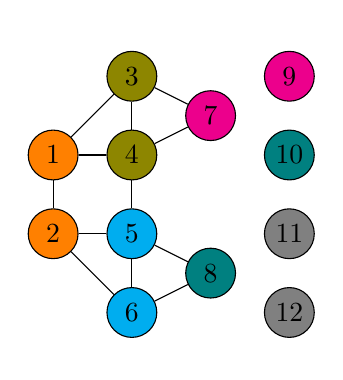
\begin{tikzpicture}
  \fill [white] (-1, -2) rectangle (1, 2) node {};  % Zentriere Graph.
  \tikzstyle{node}=[circle,draw, minimum width=18pt, inner sep=0pt, fill=white]
  \tikzstyle{color1}=[fill=orange]
  \tikzstyle{color2}=[fill=olive]
  \tikzstyle{color3}=[fill=cyan]
  \tikzstyle{color4}=[fill=magenta]
  \tikzstyle{color5}=[fill=teal]
  \tikzstyle{color6}=[fill=gray]

  \node[node, color1] (1)  at (-2, 0.5)  {$1$};
  \node[node, color1] (2)  at (-2, -0.5) {$2$};
  \node[node, color2] (3)  at (-1, 1.5)  {$3$};
  \node[node, color2] (4)  at (-1, 0.5)  {$4$};
  \node[node, color3] (5)  at (-1, -0.5) {$5$};
  \node[node, color3] (6)  at (-1, -1.5) {$6$};
  \node[node, color4] (7)  at (0,  1)    {$7$};
  \node[node, color5] (8)  at (0,  -1)   {$8$};

  \node[node, color4] (9)  at (1, 1.5)   {$9$};
  \node[node, color5] (10) at (1, 0.5)   {$10$};
  \node[node, color6] (11) at (1, -0.5)  {$11$};
  \node[node, color6] (12) at (1, -1.5)  {$12$};

  \path (1) edge (2);
  \path (1) edge (3);
  \path (1) edge (4);
  \path (2) edge (5);
  \path (2) edge (6);
  \path (3) edge (4);
  \path (3) edge (7);
  \path (4) edge (5);
  \path (4) edge (7);
  \path (5) edge (6);
  \path (5) edge (8);
  \path (6) edge (8);
\end{tikzpicture}
}
\hspace{1cm}
  \subfigure[$\gls{G}_1$]{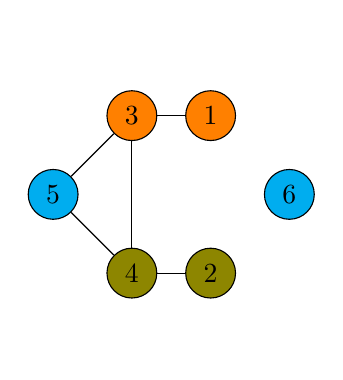
\begin{tikzpicture}
  \fill [white] (-1, -2) rectangle (1, 2) node {};  % Zentriere Graph.
  \tikzstyle{node}=[circle,draw, minimum width=18pt, inner sep=0pt, fill=white]
  \tikzstyle{color1}=[fill=orange]
  \tikzstyle{color2}=[fill=olive]
  \tikzstyle{color3}=[fill=cyan]

  \node[node, color3] (1) at (-1, 0) {$5$};
  \node[node, color1] (2) at (0,  1) {$3$};
  \node[node, color2] (3) at (0, -1) {$4$};
  \node[node, color1] (4) at (1,  1) {$1$};
  \node[node, color2] (5) at (1, -1) {$2$};

  \node[node, color3] (6) at (2, 0)  {$6$};

  \path (1) edge (2);
  \path (1) edge (3);
  \path (2) edge (3);
  \path (2) edge (4);
  \path (3) edge (5);
\end{tikzpicture}
}
\hspace{1cm}
  \subfigure[$\gls{G}_2$]{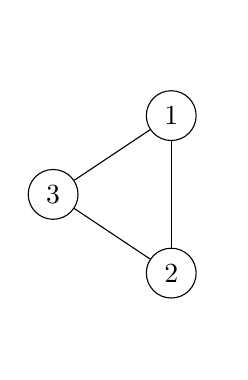
\begin{tikzpicture}
  \fill [white] (-1, -2) rectangle (1, 2) node {};  % Zentriere Graph.
  \tikzstyle{node}=[circle,draw, minimum width=18pt, inner sep=0pt, fill=white]

  \node[node] (1) at (-1,   0) {$3$};
  \node[node] (2) at (0.5,  1) {$1$};
  \node[node] (3) at (0.5, -1) {$2$};

  \path (1) edge (2);
  \path (1) edge (3);
  \path (2) edge (3);
\end{tikzpicture}
}
\hspace{1cm}
  \subfigure[Anorderung der Knoten zu einem binären Baum]{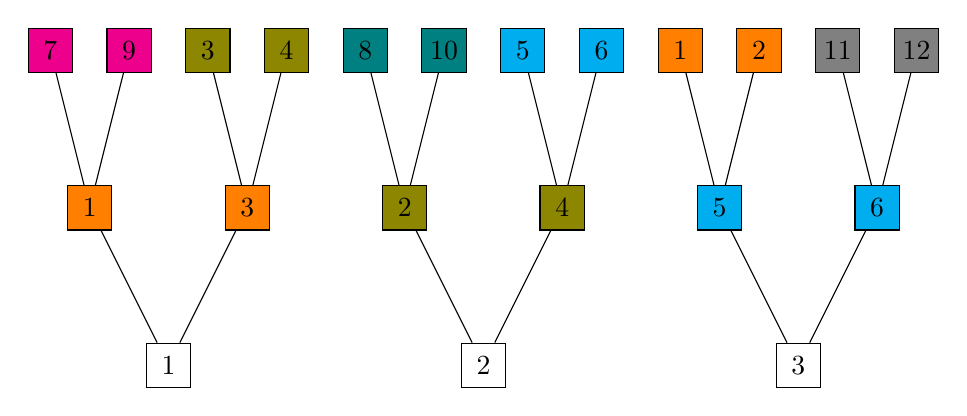
\begin{tikzpicture}
  \tikzstyle{node}=[rectangle,draw, minimum width=16pt, minimum height=16pt, inner sep=0pt, fill=white]
  \tikzstyle{color1}=[fill=orange]
  \tikzstyle{color2}=[fill=olive]
  \tikzstyle{color3}=[fill=cyan]
  \tikzstyle{color4}=[fill=magenta]
  \tikzstyle{color5}=[fill=teal]
  \tikzstyle{color6}=[fill=gray]

  \node[node, color4] (01)  at (-5.5, 2) {$7$};
  \node[node, color4] (02)  at (-4.5, 2) {$9$};
  \node[node, color2] (03)  at (-3.5, 2) {$3$};
  \node[node, color2] (04)  at (-2.5, 2) {$4$};
  \node[node, color5] (05)  at (-1.5, 2) {$8$};
  \node[node, color5] (06)  at (-0.5, 2) {$10$};
  \node[node, color3] (07)  at (0.5,  2) {$5$};
  \node[node, color3] (08)  at (1.5,  2) {$6$};
  \node[node, color1] (09)  at (2.5,  2) {$1$};
  \node[node, color1] (010) at (3.5,  2) {$2$};
  \node[node, color6] (011) at (4.5,  2) {$11$};
  \node[node, color6] (012) at (5.5,  2) {$12$};

  \node[node, color1] (11) at (-5, 0) {$1$};
  \node[node, color1] (12) at (-3, 0) {$3$};
  \node[node, color2] (13) at (-1, 0) {$2$};
  \node[node, color2] (14) at (1,  0) {$4$};
  \node[node, color3] (15) at (3,  0) {$5$};
  \node[node, color3] (16) at (5,  0) {$6$};

  \node[node] (21) at (-4, -2)  {$1$};
  \node[node] (22) at (0,  -2)  {$2$};
  \node[node] (23) at (4,  -2)  {$3$};

  \path (21) edge (11);
  \path (21) edge (12);
  \path (22) edge (13);
  \path (22) edge (14);
  \path (23) edge (15);
  \path (23) edge (16);
  \path (11) edge (01);
  \path (11) edge (02);
  \path (12) edge (03);
  \path (12) edge (04);
  \path (13) edge (05);
  \path (13) edge (06);
  \path (14) edge (07);
  \path (14) edge (08);
  \path (15) edge (09);
  \path (15) edge (010);
  \path (16) edge (011);
  \path (16) edge (012);
\end{tikzpicture}
}
\caption[Pooling auf Graphen]{Illustration einer Pooling-Operationen der Größe $4$ (\bzw{} zweier Pooling-Operationen der Größe $2$) auf einem Graphen \gls{G} der Größe $\left|\gls{V}\right| = 8$.
Das Clustering von \gls{G} liefert uns im ersten Schritt $N_1 =\left|\gls{V}_1\right| = 5$ Knoten und im darauf folgenden $N_2 = \left|\gls{V}_2\right| = 3$ Knoten.
Die Größen der Graphen werden daraufhin zu $N_2 = 3$, $N_1 = 6$ und $N_0 = 12$ angepasst, so dass jeder Knoten auf genau $2$ Vorgängerknoten verweist, indem \enquote{Fake}-Knoten zu $\gls{G}_1$ (1 Knoten) und $\gls{G}_0$ (4 Knoten) hinzugefügt werden.
Mit der Anordnung der Knoten zu einem binären Baum (d) kann die Pooling-Operation $\max\left(\cdot\right)$ eines Signals $\ve{f} \in \gls{R}^{12}$ auf $\gls{G}_0$ dann effizient als $\ve{f}_{\mathrm{pool}} \coloneqq {\left[ \max\left(\ve{f}_1, \ve{f}_2, \ve{f}_3, \ve{f}_4 \right), \max\left(\ve{f}_5, \ve{f}_6, \ve{f}_7, \ve{f}_8 \right), \max\left(\ve{f}_9, \ve{f}_{10}, \ve{f}_{11}, \ve{f}_{12} \right) \right]}^{\top} \in \gls{R}^3$ implementiert werden, wobei die Werte der \enquote{Fake}-Knoten $\ve{f}_2, \ve{f}_6, \ve{f}_{11}, \ve{f}_{12}$ auf den neutralen Wert $0$ der \gls{relu}-Aktivierungsfunktion gesetzt werden.}
\label{fig:pooling}
\end{figure}

\input{chapters/spectral/tangens}
\section{Beispiel}

Wir betrachten eine einfache $3 \times 3$ Adjazenzmatrix, d.h.\ $|\mathcal{V}| = n = 3$.

\begin{equation}
  A = \begin{pmatrix}
    0 & 1 & 0\\
    1 & 0 & 1\\
    0 & 1 & 0
  \end{pmatrix}
\end{equation}

mit Diagonalmatrix $D = \text{diag}(1, 2, 1)$.

Der Laplacian $\mathcal{L} = D - A$ ist dann

\begin{equation}
  \mathcal{L} = \begin{pmatrix}
    1 & -1 & 0\\
    -1 & 2 & -1\\
    0 & -1 & 1
  \end{pmatrix}
\end{equation}

Nun müssen die Eigenvektoren der Matrix und dessen Eigenwerte bestimmt werden, d.h.\ wir müssen das folgende Eigenwertproblem lösen

\begin{equation}
  \mathcal{L} \cdot \vec{u} = \lambda \cdot \vec{u}
\end{equation}

Wir erhalten $3$ Eigenvektoren und Eigenwerte mit

\begin{equation}
  \lambda_0 = 0, \vec{u}_0 = \frac{1}{\sqrt{3}} \begin{pmatrix}1\\1\\1\end{pmatrix} \approx \begin{pmatrix}0.58\\0.58\\0.58\end{pmatrix},
    \lambda_1 = 1, \vec{u}_1 = \frac{1}{\sqrt{2}} \begin{pmatrix}-1\\0\\1\end{pmatrix} \approx \begin{pmatrix}-0.71\\0\\0.71\end{pmatrix},
      \lambda_2 = 3, \vec{u}_2 = \frac{1}{\sqrt{6}} \begin{pmatrix}1\\-2\\1\end{pmatrix} \approx \begin{pmatrix}0.41\\-0.82\\0.41\end{pmatrix}
\end{equation}

Dann sind $U$, $\Lambda$ und $U^T$ definiert als

\begin{equation}
  U \approx \begin{pmatrix}
    0.58 & -0.71 & 0.41\\
    0.58 & 0 & -0.82\\
    0.58 & 0.71 & 0.41
  \end{pmatrix},
  \Lambda = \begin{pmatrix}
    0 & 0 & 0\\
    0 & 1 & 0\\
    0 & 0 & 3
  \end{pmatrix},
  U^T \approx \begin{pmatrix}
    0.58 & 0.58 & 0.58\\
    -0.71 & 0 & 0.71\\
    0.41 & -0.82 & 0.41
  \end{pmatrix}
\end{equation}

Angenommen wir haben ein Signal $x = {(100, 10, 1)}^T$, dann ist der Wert dieses Signals transformiert in die Fourier Domäne definiert als $\hat x \approx {(64.09, -70.00, 33.07)}^T$.
Führen wir $\hat x$ auf $x$ mittels $U \cdot \hat x$ zurück, erhalten wir korrekterweise $x = {(100, 10, 1)}^T$.

Es gilt $\lambda_{\max} = 3$
Jetzt ist $\mathbf{\tilde \Lambda}$ definiert als
\begin{equation}
  \mathbf{\tilde \Lambda} = \begin{bmatrix}
    -1 & 0 & 0\\
    0 & -\frac{1}{3} & 0\\
    0 & 0 & 1
  \end{bmatrix}
\end{equation}

Wir überprüfen die Approximation durch die Polynome mit $k = 2$:

\begin{equation}
  g_{\mathbf{\theta}}\left(\mathbf{\Lambda}\right) = \begin{pmatrix}
    1\\2\\3
  \end{pmatrix},
  g_{\mathbf{\theta}^{prime}} = \begin{pmatrix}
    wd
  \end{pmatrix}
\end{equation}

